\documentclass{IEEEconf}
\usepackage{graphicx}
\usepackage{hyperref}
\usepackage{amsmath}
\usepackage{algorithm}
\usepackage{algpseudocode}


\title{\textbf{GPU Computing} \\
    \large Project: Sparse Matrix Transposition \\
}
\author{Murtas Cristian \\ 248025 \\ cristian.murtas@studenti.unitn.it \\
\underline{\href{https://github.com/SecondarySkyler/gpu-computing/tree/main/cuda_matrix_transposition}{GitHub Repository}}
}

\begin{document}
\maketitle
\begin{abstract}
    
\end{abstract}
\section{Problem Description}
The goal of this project is to implement different algorithms to transpose sparse matrices. 
Sparce matrices are matrices in which most of the elements are zero and we are required
to utilize only those which have more than 75\% of their elements equal to zero.

The importance of this problem is due to the fact that sparse matrices are used in many fields,
such as machine learning, graphs algorithms, scientific computing and many more. Hence the ability to transpose
them efficiently is crucial.

In the following, a comparison between the implementd algorithms and the \textit{cuSparse} \cite{nvidia:cuSparse} library will be performed.
The metric used to evaluate the performance is the \textit{Effective Bandwidth}.
\section{State of the Art}
\section{Contribution and Methodology}
\subsection{Matrix Representation}
A matrix is typically represented as a 2D array, indeed, for a $m \times n$ matrix, the memory required to
store it is proportional to its size. However, for sparse matrices, a substantial reduction can be 
achieved by storying only the non-zero elements. Here we introduce the storage formats used in this project.
\subsubsection{COO Format}
The COO (Coordinate) format is the simplest way to represent a sparse matrix. It consists of three arrays:
\begin{itemize}
    \item \textbf{row\_indices}: an array of size $nnz$ containing the row index of each non-zero element.
    \item \textbf{col\_indices}: an array of size $nnz$ containing the column index of each non-zero element.
    \item \textbf{values}: an array of size $nnz$ containing the non-zero elements.
\end{itemize}
As an example, the matrix A:
\[
\begin{bmatrix}
    1 & 0 & 2 & 0 \\
    0 & 3 & 0 & 0 \\
    0 & 0 & 0 & 0 \\
    4 & 5 & 0 & 0
\end{bmatrix}
\]
Would be represented as:
\begin{align*}
    \text{row\_indices} = [0, 0, 1, 3, 3] \\
    \text{col\_indices} = [0, 2, 1, 0, 1] \\
    \text{values} = [1, 2, 3, 4, 5]
\end{align*}
\subsubsection{CSR Format}
The CSR (Compressed Sparse Row) format is similar to the COO format, indeed, it shares the \textit{values}
and the \textit{col\_indices} arrays. However, the \textit{row\_indices} array stores the locations
in the \textit{values} array that correspond to the start of each row.
Assuming the same matrix A as before, the CSR format would be:
\begin{align*}
    \text{row\_indices} = [0, 2, 3, 3, 5] \\
    \text{col\_indices} = [0, 2, 1, 0, 1] \\
    \text{values} = [1, 2, 3, 4, 5]
\end{align*}
\subsection{Algorithms}
In this section, the algorithms used to transpose the sparse matrices are presented.
First, the two algorithms based on the COO format are presented, one implemented in CUDA and the other using the \textit{cuSparse} library.
Subsequently, the algorithms that use the CSR format are shown. These algorithms take advantage of one property of the CSR format, which is that
the transpose of a CSR matrix is a CSC matrix.
\subsubsection{COO Transpose} The implementation of the COO Transpose algorithm is straightforward. It implies the swap of 
the \textit{row\_indices} and \textit{col\_indices} arrays.
It uses the shared memory to improve the performances.
\begin{algorithm}
    \caption{COO Transpose}
    \begin{algorithmic}[1]
        \Procedure{COO Transpose}{$rows, cols, nnz$}
            \State $sharedRows[BLOCK\_SIZE]$
            \State $sharedCols[BLOCK\_SIZE]$
            \State $tid \gets blockIdx.x * blockDim.x + threadIdx.x$
            \If{$tid < nnz$}
                \Comment Copy to shared memory
                \State $sharedRows[threadIdx.x] \gets rows[tid]$
                \State $sharedCols[threadIdx.x] \gets cols[tid]$
                \State $\_\_syncthreads()$
                \State $temp \gets sharedRows[threadIdx.x]$
                \State $sharedRows[threadIdx.x] \gets sharedCols[threadIdx.x]$
                \State $sharedCols[threadIdx.x] \gets temp$
                \State $\_\_syncthreads()$
                \State $rows[tid] \gets sharedRows[threadIdx.x]$
                \State $cols[tid] \gets sharedCols[threadIdx.x]$
            \EndIf
        \EndProcedure
    \end{algorithmic}
\end{algorithm}
\subsubsection{cuSparse COO Transpose} Unfortunately, the \textit{cuSparse} library does not provide a direct way to
transpose a COO matrix. However, it is possible to use the \textit{cusparseSpMM} \cite{cusparse:spmm} function to perform a matrix multiplication
between a sparse matrix and a dense matrix. This function, allows to specify an operation (\textit{TRANSPOSE} or \textit{CONJUGATE\_TRANSPOSE})
to perform on the matrices, before the multiplication. By using one of the fundamental 
properties of the identity matrix, which states that given the identity matrix $I$: \\
\[
    I \cdot A = A 
\]
It is possible to transpose the matrix by applying the \textit{TRANSPOSE} operation on the sparse matrix and multiplying it with the identity matrix.
\subsubsection{CSR Transpose}
The CSR transposition requires the following steps:
\begin{itemize}
    \item count the number of non-zero elements in each column;
    \item perform an exclusive scan to construct the \textit{col\_pointers} array.
    \item fill the \textit{row\_indices}  and \textit{values} arrays.
\end{itemize}
Following this separation, three kernels, one for each step, have been implemented.
Thanks to this modularity, it has been possible to test each step individually and compare the results of the different implementations.
Indeed, two versions of the algorithm have been implemented, both shares the first and the third kernel but differ in the second one. \\
\paragraph{Count Non-Zero Elements}
This kernel counts the occurrences of each column in the \textit{col\_indices} array. 
The \textit{atomicAdd} function performs an atomic addition on the \textit{cscColPtr} array.
\begin{algorithm}
    \caption{Count Non-Zero Elements}
    \begin{algorithmic}
        \Procedure{Count NNZ}{$nnz, csrColIdx, cscColPtr$}
            \State $sharedCsrCols[BLOCK\_SIZE]$
            \State $tid \gets blockIdx.x * blockDim.x + threadIdx.x$
            \State $sharedCsrCols[threadIdx.x] \gets csrColIdx[tid]$
            \State $\_\_syncthreads()$
            \If{$tid < nnz$}
                \State $col \gets sharedCsrCols[threadIdx.x]$
                \State $atomicAdd(cscColPtr[col + 1], 1)$
            \EndIf
        \EndProcedure
    \end{algorithmic}
\end{algorithm}
\paragraph{Scan (version 1)}
The na\"ive approach to perform the scan operation is to use a single thread which iterates over the array and performs the exclusive scan.
\begin{algorithm}
    \caption{Scan with 1 thread}
    \begin{algorithmic}
        \Procedure{Scan}{$n, cscColPtr$}
            \State $tid \gets blockIdx.x * blockDim.x + threadIdx.x$
            \If{$tid == 0$}
                \State $cscColPtr[0] \gets 0$
                \For{$i \gets 1$ \textbf{to} $n$}
                    \State $cscColPtr[i] += cscColPtr[i - 1]$
                \EndFor
            \EndIf
        \EndProcedure
    \end{algorithmic}
\end{algorithm}
\paragraph{Scan (version 2)}
The second version of the scan algorithm takes inspiration from what has been explained in the book \textit{GPU Gems 3} \cite{nvidia:gpu_gems_3}.
More in detail, in chapter 39.2.4\footnote{\href{https://developer.nvidia.com/gpugems/gpugems3/part-vi-gpu-computing/chapter-39-parallel-prefix-sum-scan-cuda}{Chapter 39.2.4}},
the authors present a parallel implementation which works on arrays of arbitrary size.
Figure \ref{fig:scan_la} shows the idea behind the algorithm. \\
To achieve this, the procedure is divided into two steps:
\begin{itemize}
    \item Perform a scan on the array using a block-wide scan algorithm. Store the sum of each block in a separate array;
    \item Perform a scan on the auxiliary array. Add the sum of the auxiliary array blocks to the elements of the original array.
\end{itemize}
As before these two steps have been implemented in two separate kernels, first an exclusive scan (Algorithm \ref{alg:scan_v2})
followed by a uniform update (Algorithm \ref{alg:uniform_update}).
\begin{figure}
    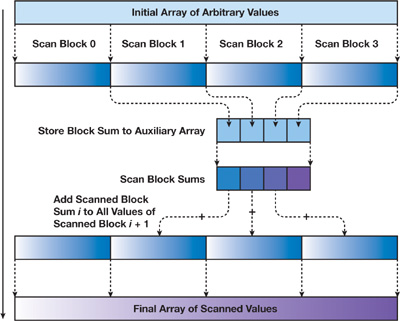
\includegraphics[width=\columnwidth]{images/scan_la.jpg}
    \caption{Algorithm for Performing a Sum Scan on a Large Array of Values}
    \label{fig:scan_la}
\end{figure}
\begin{algorithm}
    \caption{Scan with multiple threads}
    \begin{algorithmic}
        \Procedure{Scan}{$cscColPtr, auxBlocks, cols$}
            \State $tid \gets blockIdx.x * blockDim.x + threadIdx.x$
            \State $bid \gets blockDim.x$
            \State $block[BLOCK\_SIZE]$
            \Comment Copy the cscColPtr array into the shared memory
            
            \For{$stride \gets 1$ \textbf{to} $BLOCK\_SIZE$}
                \State $index \gets (tid+1) * stride * 2 - 1$
                \If{$index < BLOCK\_SIZE$}
                    \State $block[index] += block[index - stride]$
                \EndIf
                \State $stride *=2$
            \EndFor

            \State $\_\_syncthreads()$

            \For{$stride \gets BLOCK\_SIZE$ \textbf{until} $stride > 0$}
                \State $index \gets (tid+1) * stride * 2 - 1$
                \If{$index + stride < BLOCK\_SIZE$}
                    \State $block[index + stride] += block[index]$
                \EndIf
                \State $stride /= 2$
            \EndFor

            \State $\_\_syncthreads()$

            \If{$tid < cols$}
                \State $cscColPtr[tid] \gets block[threadIdx.x]$
            \EndIf

            \If{$tid == BLOCK\_SIZE - 1$}
                \State $auxBlocks[blockIdx.x] \gets block[tid]$
            \EndIf
        \EndProcedure
    \end{algorithmic}
    \label{alg:scan_v2}
\end{algorithm}
\begin{algorithm}
    \caption{Uniform Update}
    \begin{algorithmic}
        \Procedure{Update}{$cscColPtr, auxBlocks, cols$}
        \State $bid \gets blockIdx.x$
        \State $idx \gets blockIdx.x * blockDim.x + threadIdx.x$
        \If{$bid > 0$ }
            \State $cscColPtr[idx] += auxBlocks[bid - 1]$
        \EndIf
        \EndProcedure
    \end{algorithmic}
    \label{alg:uniform_update}
\end{algorithm}
\paragraph{Fill}
This step has the purpose of filling the \textit{csc\_row\_indices} and \textit{csc\_values} arrays.
The kernel is straightforward, it iterates over the \textit{csr\_row\_indices} array and for each element,
it increments the corresponding element in the \textit{csc\_col\_ptr} array and stores the row index and
the value in the \textit{csc\_row\_indices} and \textit{csc\_values} arrays.
% TODO fix this algorithm because it exceed the page
\begin{algorithm}
    \caption{Fill CSC Row and Values}
    \begin{algorithmic}
        \Procedure{Fill}{$rows, cscColPtr, csrRowIdx, csrColIdx, csrValues, cscValues, cscRowIdx$}
            \State $tid \gets blockIdx.x * blockDim.x + threadIdx.x$
            \If{$tid < rows$}
                \For{$j = csrRowIdx[tid]$ \textbf{to} $j < csrRowIdx[tid+1]$}
                    \State $col \gets csrColIdx[j]$
                    \State $idx \gets atomicAdd(cscColPtr[col], 1)$
                    \State $cscRowIdx[idx] \gets tid$
                    \State $cscValues[idx] \gets csrValues[j]$
                \EndFor
            \EndIf
        \EndProcedure
    \end{algorithmic}
\end{algorithm}
\subsubsection{cuSparse CSR Transpose}
The \textit{cuSparse} library provides the \textit{cusparseCsr2cscEx2} function \cite{cusparse:csr2cscex2}, thanks to which
it is possible to transpose a CSR matrix.
\section{Experiments and System Description}
The entire experiment has been conducted on the Marzola cluster of the University of Trento, 
which is equipped with NVIDIA A30 GPUs \cite{nvidia:a30}.
Furthermore, the code has also been tested on a local machine equipped with an NVIDIA RTX 3070 \cite{nvidia:rtx3070}.
For both setup, the information about the GPUs have been retrieved using the \textit{cudaGetDeviceProperties} function \cite{nvidia:cudaDeviceProp}.
The code has been compiled using CUDA 12.1.
\subsection{Experiments Setup}
In order to evaluate the performance of the implemented algorithms, ten matrices from the \textit{SuiteSparse} \cite{spm:suitesparse} collection
have been selected. The matrices have been chosen to be squared and non-symmetric\footnote{The list of used matrices is available in the \href{https://github.com/SecondarySkyler/gpu-computing-project}{README}}. \\
The execution of the kernels has been repeated 100 times to improve the accuracy of the measurements. The metric used to evaluate the performance is the \textit{Effective Bandwidth} which has 
been calculated accordingly to the algorithm used.
\section{Results}
\begin{table}[h]
    \begin{tabular}{|ccc|}
    \hline
    \multicolumn{3}{|c|}{\textbf{COO Transposition Results}}                                               \\ \hline
    \multicolumn{1}{|l|}{}                      & \multicolumn{2}{c|}{\textbf{Effective Bandwidth (GB/s)}} \\ \hline
    \multicolumn{1}{|c|}{\textbf{Matrix Names}} & \multicolumn{1}{c|}{Own COO}        & cuSparse COO       \\ \hline
    \multicolumn{1}{|c|}{arc130}                & \multicolumn{1}{c|}{4.53}           & 1.58               \\ \hline
    \multicolumn{1}{|c|}{fd15}                  & \multicolumn{1}{c|}{143.54}         & 352.47             \\ \hline
    \multicolumn{1}{|c|}{bips07\_1998}          & \multicolumn{1}{c|}{188.39}         & 281.82             \\ \hline
    \multicolumn{1}{|c|}{bayer10}               & \multicolumn{1}{c|}{254.33}         & N/A                \\ \hline
    \multicolumn{1}{|c|}{piston}                & \multicolumn{1}{c|}{268.42}         & 28.52              \\ \hline
    \multicolumn{1}{|c|}{cage10}                & \multicolumn{1}{c|}{348.07}         & 112.43             \\ \hline
    \multicolumn{1}{|c|}{Ill\_Stokes}           & \multicolumn{1}{c|}{405.91}         & 60.44              \\ \hline
    \multicolumn{1}{|c|}{msc10848}              & \multicolumn{1}{c|}{686.96}         & 36.98              \\ \hline
    \multicolumn{1}{|c|}{appu}                  & \multicolumn{1}{c|}{838.66}         & 4.43               \\ \hline
    \multicolumn{1}{|c|}{TSOPF\_RS\_b300\_c2}   & \multicolumn{1}{c|}{725.79}         & 19.81              \\ \hline
    \end{tabular}
    \caption{COO Transposition Results}
    \label{tab:coo_results}
\end{table}
\begin{table}[h]
    \begin{tabular}{|cccc|}
    \hline
    \multicolumn{4}{|c|}{\textbf{CSR Transposition Results}}                                                          \\ \hline
    \multicolumn{1}{|l|}{}                      & \multicolumn{3}{c|}{\textbf{Effective Bandwidth (GB/s)}}            \\ \hline
    \multicolumn{1}{|c|}{\textbf{Matrix Names}} & \multicolumn{1}{c|}{v1}    & \multicolumn{1}{c|}{v2}     & cuSparse \\ \hline
    \multicolumn{1}{|c|}{arc130}                & \multicolumn{1}{c|}{0.97}  & \multicolumn{1}{c|}{0.95}   & 0.26     \\ \hline
    \multicolumn{1}{|c|}{fd15}                  & \multicolumn{1}{c|}{8.25}  & \multicolumn{1}{c|}{88.59}  & 14.10    \\ \hline
    \multicolumn{1}{|c|}{bips07\_1998}          & \multicolumn{1}{c|}{8.60}  & \multicolumn{1}{c|}{72}     & 11.14    \\ \hline
    \multicolumn{1}{|c|}{bayer10}               & \multicolumn{1}{c|}{13.64} & \multicolumn{1}{c|}{111.47} & 33.55    \\ \hline
    \multicolumn{1}{|c|}{piston}                & \multicolumn{1}{c|}{42.15} & \multicolumn{1}{c|}{66.71}  & 16.76    \\ \hline
    \multicolumn{1}{|c|}{cage10}                & \multicolumn{1}{c|}{23.23} & \multicolumn{1}{c|}{112.75} & 25.06    \\ \hline
    \multicolumn{1}{|c|}{Ill\_Stokes}           & \multicolumn{1}{c|}{16.95} & \multicolumn{1}{c|}{126.61} & 60.41    \\ \hline
    \multicolumn{1}{|c|}{msc10848}              & \multicolumn{1}{c|}{55.44} & \multicolumn{1}{c|}{97.42}  & 84.70    \\ \hline
    \multicolumn{1}{|c|}{appu}                  & \multicolumn{1}{c|}{80.75} & \multicolumn{1}{c|}{128.17} & 146.83   \\ \hline
    \multicolumn{1}{|c|}{TSOPF\_RS\_b300\_c2}   & \multicolumn{1}{c|}{75.39} & \multicolumn{1}{c|}{96.94}  & 199.16   \\ \hline
    \end{tabular}
    \caption{CSR Transposition Results}
    \label{tab:csr_results}
\end{table}
\section{Conclusions}

\clearpage
\bibliographystyle{plain}
\bibliography{references}
\end{document}